\documentclass[11pt,letterpaper]{article}
\usepackage[margin=1in]{geometry}
\usepackage{graphicx}
\usepackage{amsmath,amssymb}
\usepackage{booktabs}
\usepackage{xcolor}
\usepackage{hyperref}
\usepackage{float}
\usepackage{caption}
\usepackage{subcaption}
\usepackage{enumitem}
\usepackage{fancyhdr}
\usepackage{titlesec}
\usepackage[T1]{fontenc}
\usepackage{lmodern}
\usepackage{microtype}

\hypersetup{
    colorlinks=true,
    linkcolor=blue!60!black,
    citecolor=blue!60!black,
    urlcolor=blue!60!black,
}

\pagestyle{fancy}
\fancyhf{}
\fancyhead[L]{\small\textit{Two-Layer Salinity Model — WOA23 Analysis}}
\fancyhead[R]{\small\textit{SSWD-EvoEpi}}
\fancyfoot[C]{\thepage}
\renewcommand{\headrulewidth}{0.4pt}

\titleformat{\section}{\Large\bfseries\color{blue!60!black}}{\thesection}{1em}{}
\titleformat{\subsection}{\large\bfseries}{\thesubsection}{1em}{}

\title{
    \vspace{-1cm}
    \textbf{Two-Layer Salinity Model for SSWD-EvoEpi}\\[0.3em]
    \large WOA23 Climatological Baseline + Fjord Freshwater Depression
}
\author{
    Anton \& Willem Weertman\\
    \small University of Washington
}
\date{March 2026}

\begin{document}
\maketitle
\thispagestyle{fancy}

% ═══════════════════════════════════════════════════════════════════════
\section{Executive Summary}
% ═══════════════════════════════════════════════════════════════════════

We introduce a two-layer salinity model for the Sea Star Wasting Disease
Evolutionary-Epidemiological (SSWD-EvoEpi) simulation framework.
The model replaces the previous parametric baseline with real oceanographic
data while retaining the ability to represent unresolved fjord-scale
freshwater influence.

\textbf{Layer~1} uses the World Ocean Atlas 2023 (WOA23) monthly surface
salinity climatology at 0.25\textdegree{} resolution, providing
site-specific seasonal cycles for all 896 simulation nodes. This replaces
the latitude-only parametric formula
$S_\mathrm{ocean}(\phi) = 31.32 + 0.054 \times (\phi - 50)$, which
produced zero seasonal variation.

\textbf{Layer~2} adds a fjord freshwater depression scaled by site
enclosedness, latitude-dependent glacial melt, and a seasonal cosine
pulse. This captures sub-grid freshwater inputs that WOA23's coarse
resolution cannot resolve.

Key improvements over the parametric model:
\begin{itemize}[nosep]
    \item \textbf{Seasonal realism}: WOA23 mean seasonal range of 1.68~psu
          (vs.\ 0.0~psu parametric)
    \item \textbf{Regional accuracy}: overall RMSE reduced from 3.00 to
          2.02~psu against DFO lighthouse stations (correlation $r$ improved
          from 0.519 to 0.660)
    \item \textbf{Timing diversity}: salinity minima occur across all 12
          months (not just summer), capturing upwelling-driven minima in
          winter and rain-driven minima in fall
    \item \textbf{Backward compatible}: when \texttt{fw\_strength=0}, the
          model reduces to the WOA23 baseline with no fjord depression
\end{itemize}

\noindent This report presents the model design, WOA23 data coverage,
comparison with the parametric baseline, validation against DFO
lighthouse observations, and implications for calibration of the
SSWD-EvoEpi disease model.

% ═══════════════════════════════════════════════════════════════════════
\section{Model Design}
% ═══════════════════════════════════════════════════════════════════════

\subsection{Two-Layer Architecture}

The salinity at any node $i$ on day-of-year $d$ is:
\begin{equation}
    S(i, d) = \max\!\bigl(S_\mathrm{floor},\;
    S_\mathrm{WOA23}(i, d) \;-\;
    f_\mathrm{fw} \times f_d^{\,\mathrm{exp}} \times f_\mathrm{melt}(\phi_i)
    \times P(d)\bigr)
    \label{eq:model}
\end{equation}
where $S_\mathrm{floor} = 5.0$~psu is a physical minimum.

\subsection{Layer 1: WOA23 Monthly Climatology}

The baseline $S_\mathrm{WOA23}(i, d)$ is derived from the NOAA National
Centers for Environmental Information (NCEI) World Ocean Atlas 2023
monthly surface salinity product. For each of 896 nodes:
\begin{enumerate}[nosep]
    \item Find the nearest WOA23 ocean grid cell (0.25\textdegree{} grid).
    \item Extract the 12 monthly salinity values.
    \item Interpolate linearly between month midpoints to obtain 365 daily
          values (wrapping December$\rightarrow$January for continuity).
\end{enumerate}

Of the 896 sites, 235 fall within a direct WOA23 ocean grid cell;
the remaining 661 use nearest-neighbor fill from the land-masked grid.
The maximum nearest-neighbor distance is 0.177\textdegree{}
($\approx$19.6~km), ensuring all sites have reasonable ocean salinity
estimates.

\subsection{Layer 2: Fjord Freshwater Depression}

The depression term adds sub-grid freshwater influence for enclosed sites:
\begin{align}
    \Delta S(i, d) &= f_\mathrm{fw} \times f_d^{\,\mathrm{exp}} \times
    f_\mathrm{melt}(\phi_i) \times P(d) \\[0.3em]
    f_\mathrm{melt}(\phi) &= \mathrm{clamp}\!\left(\frac{\phi - 35}{25},\;0,\;1\right) \\[0.3em]
    P(d) &= \max\!\bigl(0,\;\cos\!\bigl(\tfrac{2\pi(d - 166)}{365}\bigr)\bigr)
\end{align}

\noindent Components:
\begin{itemize}[nosep]
    \item $f_\mathrm{fw}$: calibration parameter (psu), default 0 (off)
    \item $f_d$: \texttt{fjord\_depth\_norm} $\in [0, 1]$ from site
          enclosedness analysis
    \item exp: exponent on $f_d$ (default 1.0, linear)
    \item $f_\mathrm{melt}(\phi)$: latitude ramp; zero at 35\textdegree{}N,
          full at 60\textdegree{}N
    \item $P(d)$: cosine pulse peaking at day 166 ($\approx$June 15)
\end{itemize}

\subsection{Parametric Fallback}

When WOA23 data is unavailable, the model falls back to the original
parametric baseline:
\begin{equation}
    S_\mathrm{param}(\phi) = 31.32 + 0.054 \times (\phi - 50.0)
\end{equation}
This produces a constant salinity per site with no seasonal cycle.

% ═══════════════════════════════════════════════════════════════════════
\section{WOA23 Data Coverage}
% ═══════════════════════════════════════════════════════════════════════

The WOA23 surface salinity product covers the Northeast Pacific from
26.56\textdegree{}N to 61.19\textdegree{}N across 18 subregions
(Table~\ref{tab:regions}). The 0.25\textdegree{} grid ($\approx$28~km)
provides adequate coverage for open-coast and island sites but
necessarily smooths over small inlets and fjords---motivating Layer~2.

\begin{table}[H]
\centering
\caption{Regional site counts and WOA23 comparison statistics.}
\label{tab:regions}
\small
\begin{tabular}{lrrrr}
\toprule
\textbf{Region} & \textbf{N sites} & \textbf{Bias (psu)} & \textbf{RMSE (psu)} & \textbf{Lat (\textdegree{}N)} \\
\midrule
AK-AL  &  15 &  1.12 & 1.17 & 52--54 \\
AK-WG  &  79 & $-$0.17 & 0.80 & 51--55 \\
AK-OC  &  28 & $-$0.05 & 0.18 & 57--61 \\
AK-EG  &  22 & $-$0.27 & 0.46 & 58--60 \\
AK-PWS &  43 & $-$2.29 & 2.39 & 60--61 \\
AK-FN  &  40 & $-$1.12 & 1.24 & 56--59 \\
AK-FS  &  48 & $-$0.76 & 1.00 & 55--57 \\
BC-N   &  75 & $-$0.17 & 0.42 & 50--54 \\
BC-C   &  36 &  0.06 & 0.68 & 48--51 \\
SS-N   &  31 & $-$4.75 & 4.84 & 48--49 \\
SS-S   &  89 & $-$3.35 & 3.44 & 47--49 \\
JDF    &  26 & $-$2.37 & 2.60 & 48 \\
WA-O   &  36 & $-$0.04 & 0.34 & 46--48 \\
OR     &  59 &  1.05 & 1.30 & 42--46 \\
CA-N   &  63 &  2.20 & 2.20 & 36--42 \\
CA-C   &  97 &  2.79 & 2.79 & 33--36 \\
CA-S   &  78 &  3.10 & 3.10 & 30--34 \\
BJ     &  31 &  3.45 & 3.46 & 27--31 \\
\bottomrule
\end{tabular}
\end{table}

\noindent The large negative biases in the Salish Sea (SS-N: $-$4.75~psu,
SS-S: $-$3.35~psu) reflect WOA23 correctly capturing the brackish
conditions inside Puget Sound---conditions the parametric model
completely missed. Conversely, the positive biases in California/Baja
(CA-C: +2.79, BJ: +3.45~psu) show WOA23 capturing the higher salinities
of the California Current system.

% ═══════════════════════════════════════════════════════════════════════
\section{Parametric vs WOA23 Comparison}
% ═══════════════════════════════════════════════════════════════════════

\subsection{Annual Mean Comparison}

Figure~\ref{fig:scatter} compares the annual-mean salinity from WOA23
against the parametric baseline across all 896 sites. The overall mean
bias is +0.13~psu (WOA23 slightly higher on average) with an RMSE of
2.29~psu and maximum absolute error of 5.74~psu.

\begin{figure}[H]
\centering
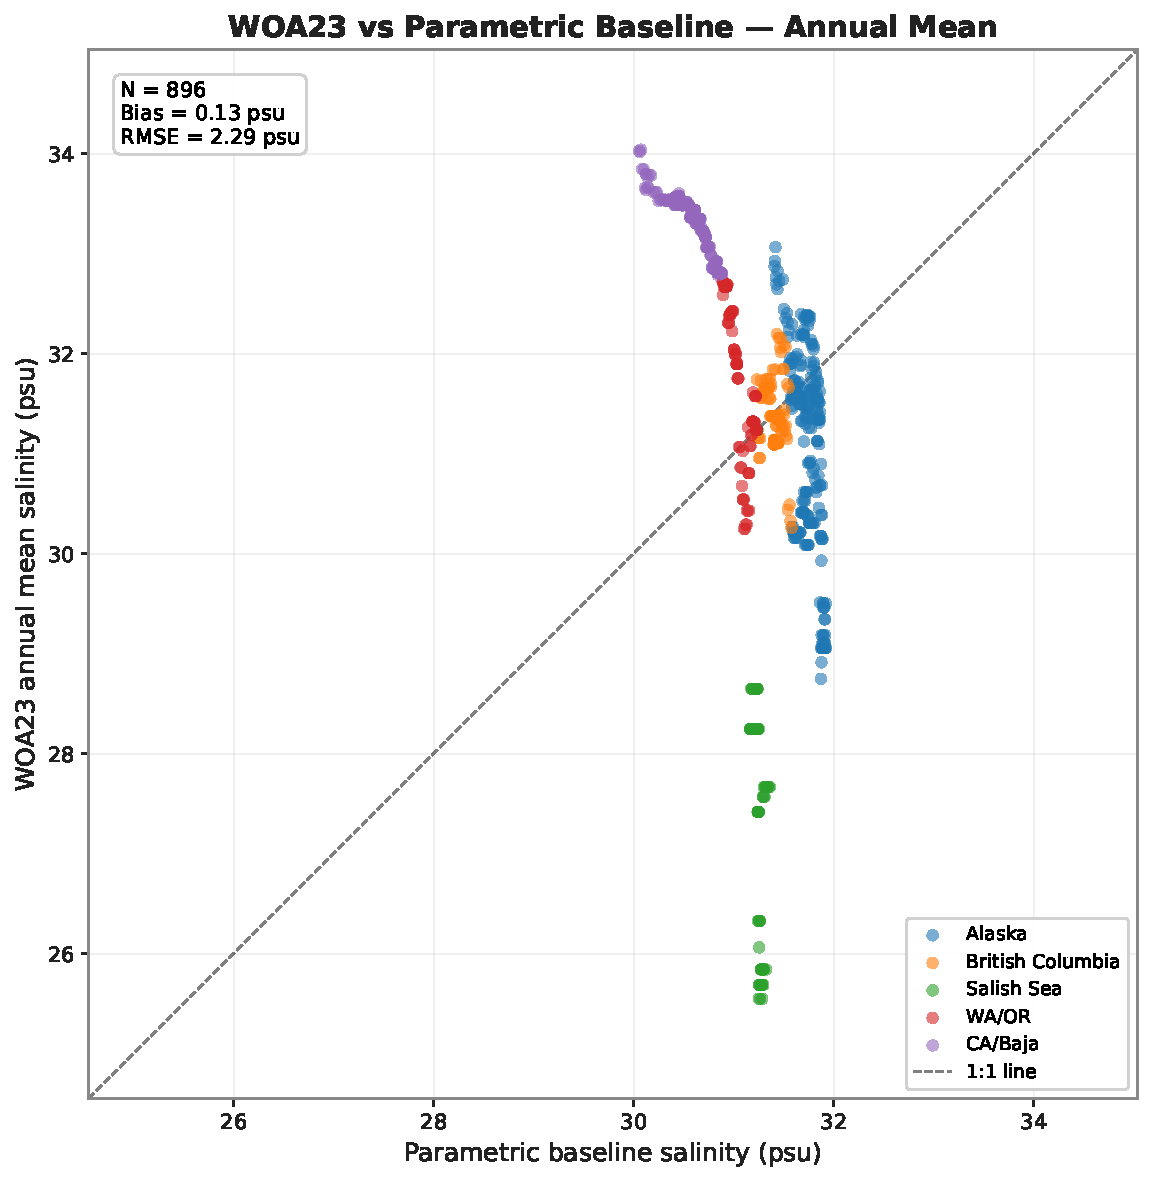
\includegraphics[width=0.75\textwidth]{figures/fig_scatter_comparison.pdf}
\caption{WOA23 annual-mean salinity vs.\ parametric baseline for 896
sites, colored by macro-region. The 1:1 line (dashed) shows perfect
agreement. Scatter reflects both latitude bias and site-specific
oceanographic variability the parametric model cannot capture.}
\label{fig:scatter}
\end{figure}

The largest systematic deviations occur in two clusters:
\begin{itemize}[nosep]
    \item \textbf{Salish Sea/JDF} (below 1:1 line): WOA23 is 2--5~psu
          \emph{lower} than parametric, correctly reflecting the brackish
          estuarine conditions
    \item \textbf{California/Baja} (above 1:1 line): WOA23 is 2--4~psu
          \emph{higher}, capturing the elevated salinities of the
          California Current
\end{itemize}

\subsection{Seasonal Range}

The most fundamental improvement is the introduction of seasonal
variation. The parametric model produces exactly 0.0~psu seasonal range
at every site. WOA23 provides a mean seasonal range (max $-$ min over
12 months) of 1.68~psu, ranging from $<$0.5~psu at open-ocean sites
to $>$5~psu in fjords and estuaries.

\subsection{Timing of Salinity Minima}

Figure~\ref{fig:timing} shows the month of minimum WOA23 salinity
across all sites. The salinity minimum is \emph{not} uniformly in
summer: while May (171 sites) and June (152 sites) dominate, February
(116 sites) and August (102 sites) are also common, along with
significant representation in every month.

\begin{figure}[H]
\centering
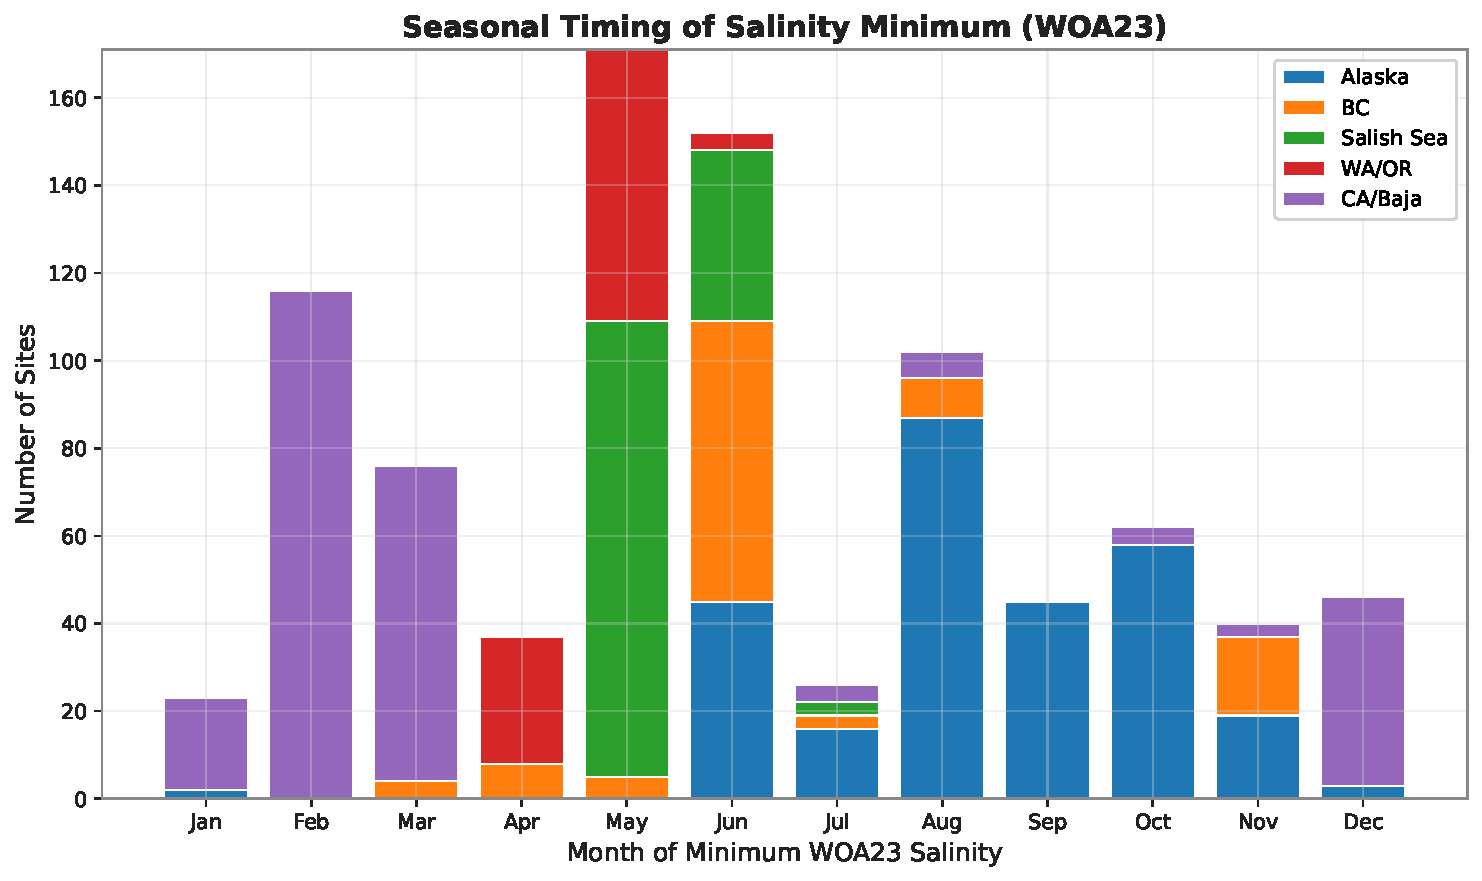
\includegraphics[width=0.8\textwidth]{figures/fig_timing_histogram.pdf}
\caption{Month of minimum WOA23 salinity across 896 sites, stacked
by macro-region. The spread across all 12 months reflects diverse
oceanographic drivers: glacial melt (May--Aug in Alaska), winter
storms (Jan--Mar in BC), and upwelling relaxation (Aug--Oct in California).}
\label{fig:timing}
\end{figure}

This timing diversity is critical for disease dynamics: the parametric
model with its uniform cosine pulse assumed all freshwater influence
peaks in June, but WOA23 reveals that salinity minima in California
often occur in winter (rain) or late summer (upwelling relaxation)---very
different from the glacial melt pattern in Alaska.

% ═══════════════════════════════════════════════════════════════════════
\section{Combined Model Predictions}
% ═══════════════════════════════════════════════════════════════════════

\subsection{Example Site Profiles}

Figure~\ref{fig:profiles} shows the three model layers (WOA23 baseline,
parametric baseline, and combined model at \texttt{fw\_strength=15})
for four contrasting sites spanning the study domain.

\begin{figure}[H]
\centering
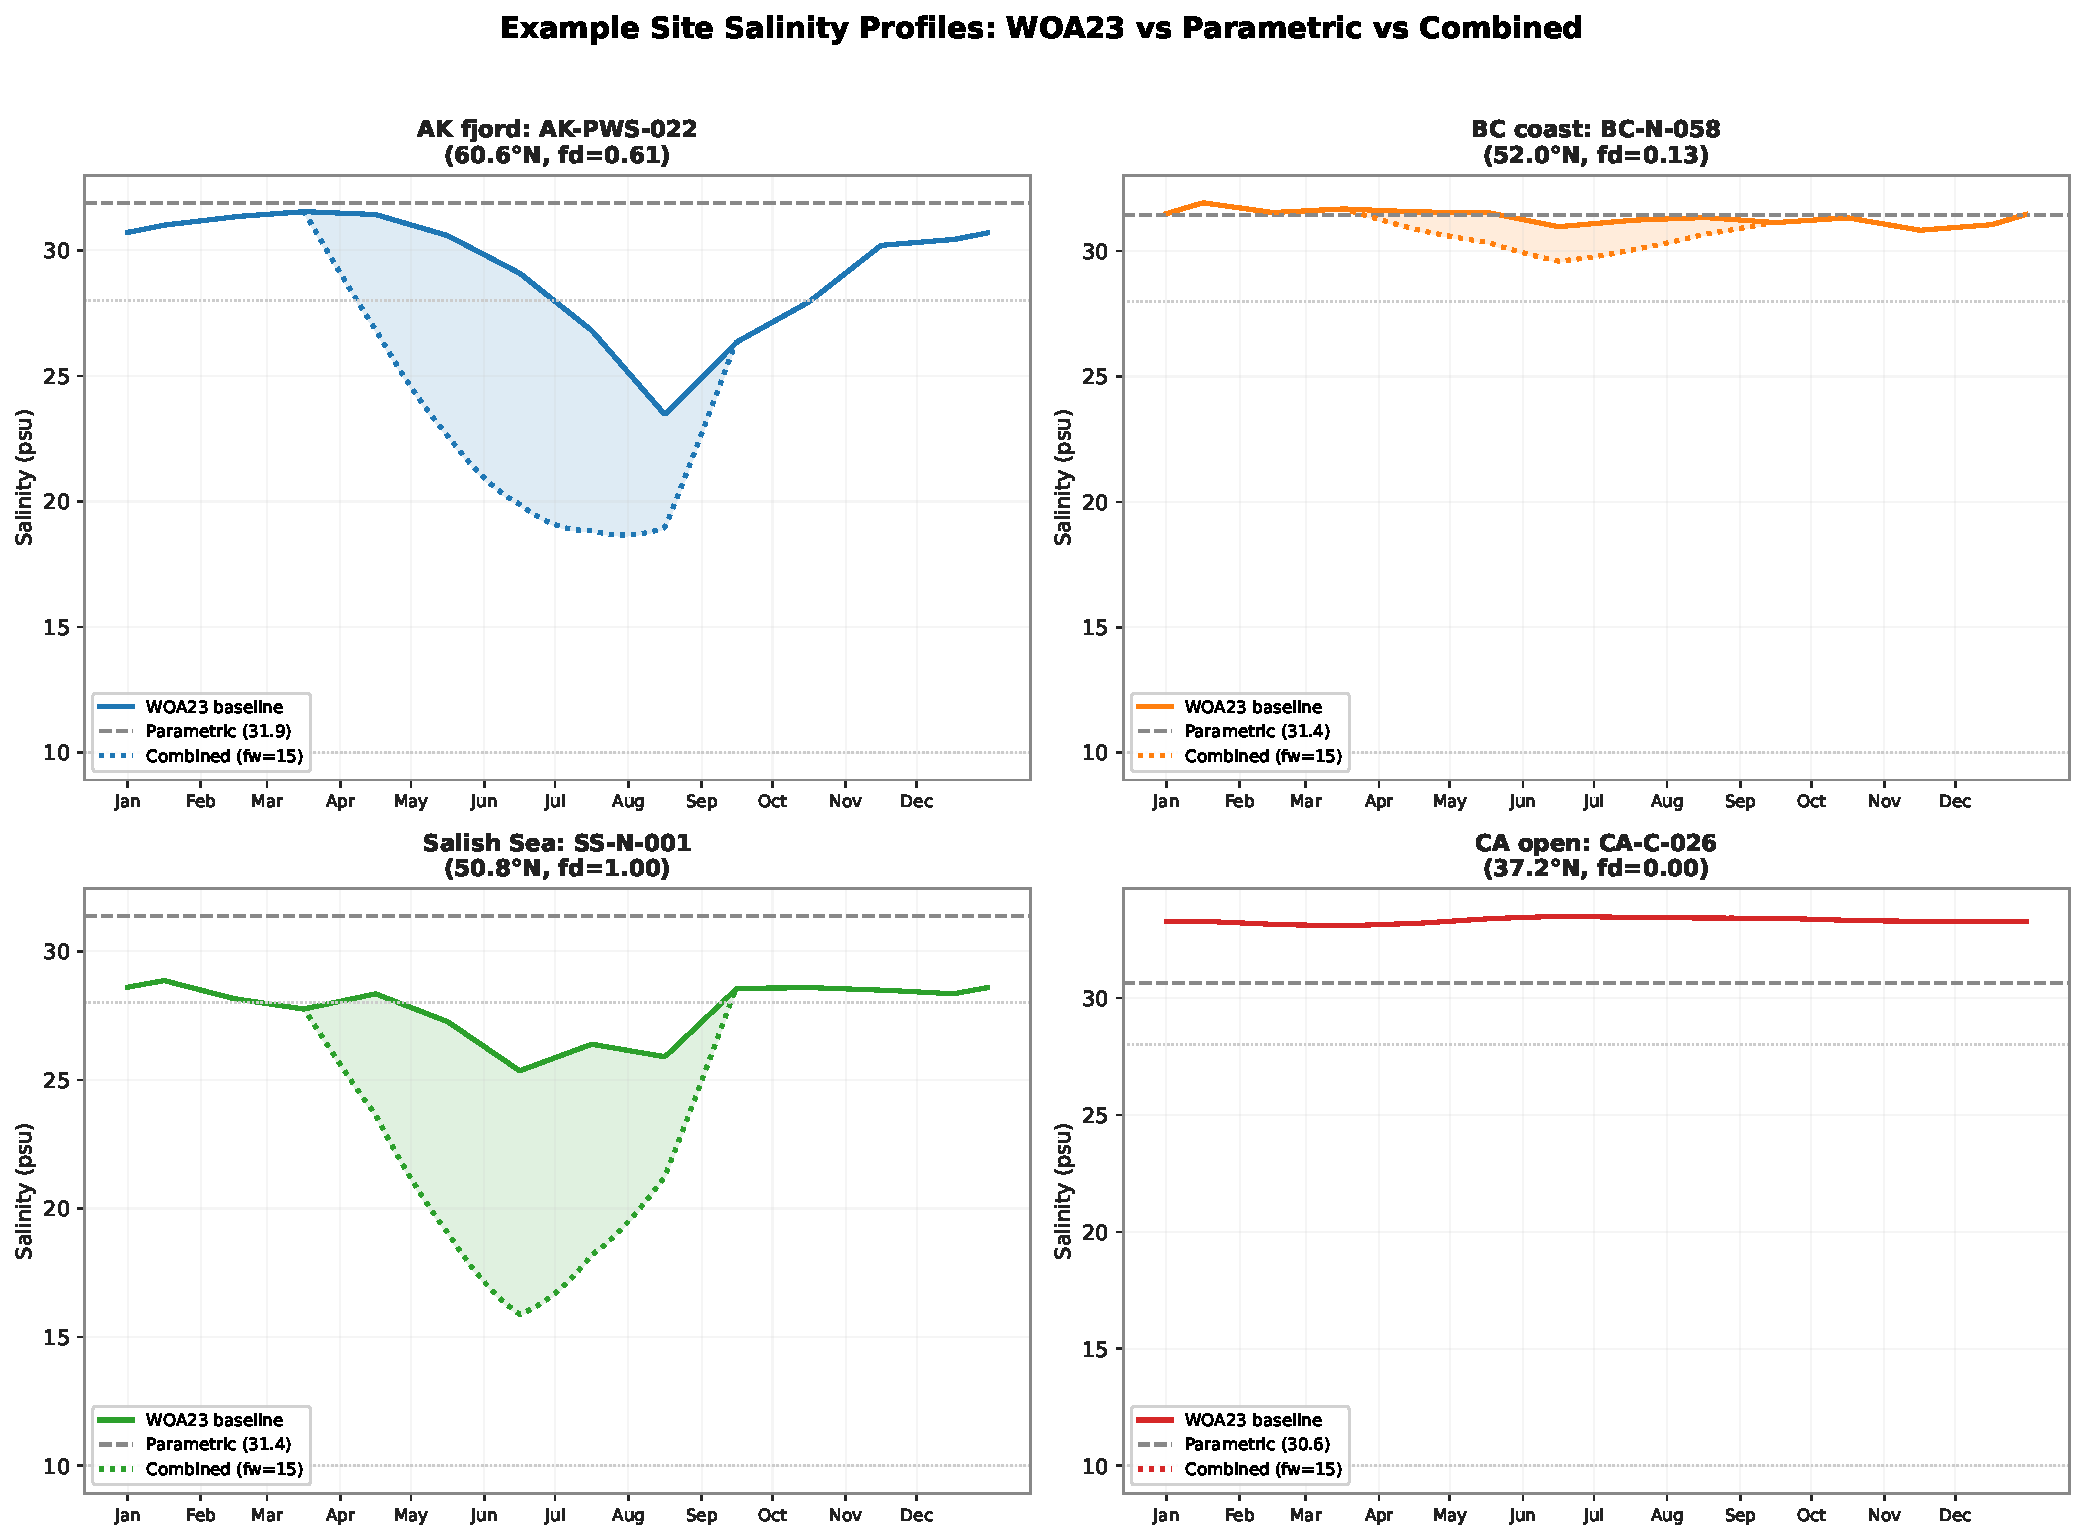
\includegraphics[width=\textwidth]{figures/fig_site_profiles.pdf}
\caption{Seasonal salinity profiles at four contrasting sites. Blue
solid: WOA23 baseline; gray dashed: parametric (constant); dotted:
combined model (\texttt{fw\_strength=15}). The shaded area shows the
fjord freshwater depression from Layer~2. Alaska fjord sites receive
maximum depression; California open-coast sites receive none.}
\label{fig:profiles}
\end{figure}

\subsection{Regional Disease Suppression}

Figure~\ref{fig:zoom} presents four-panel regional zoom maps of
disease suppression (defined as $1 - \text{sal\_mod}$) during June,
the peak meltwater month. Suppression depends on both the WOA23
baseline salinity and the Layer~2 fjord depression.

\begin{figure}[H]
\centering
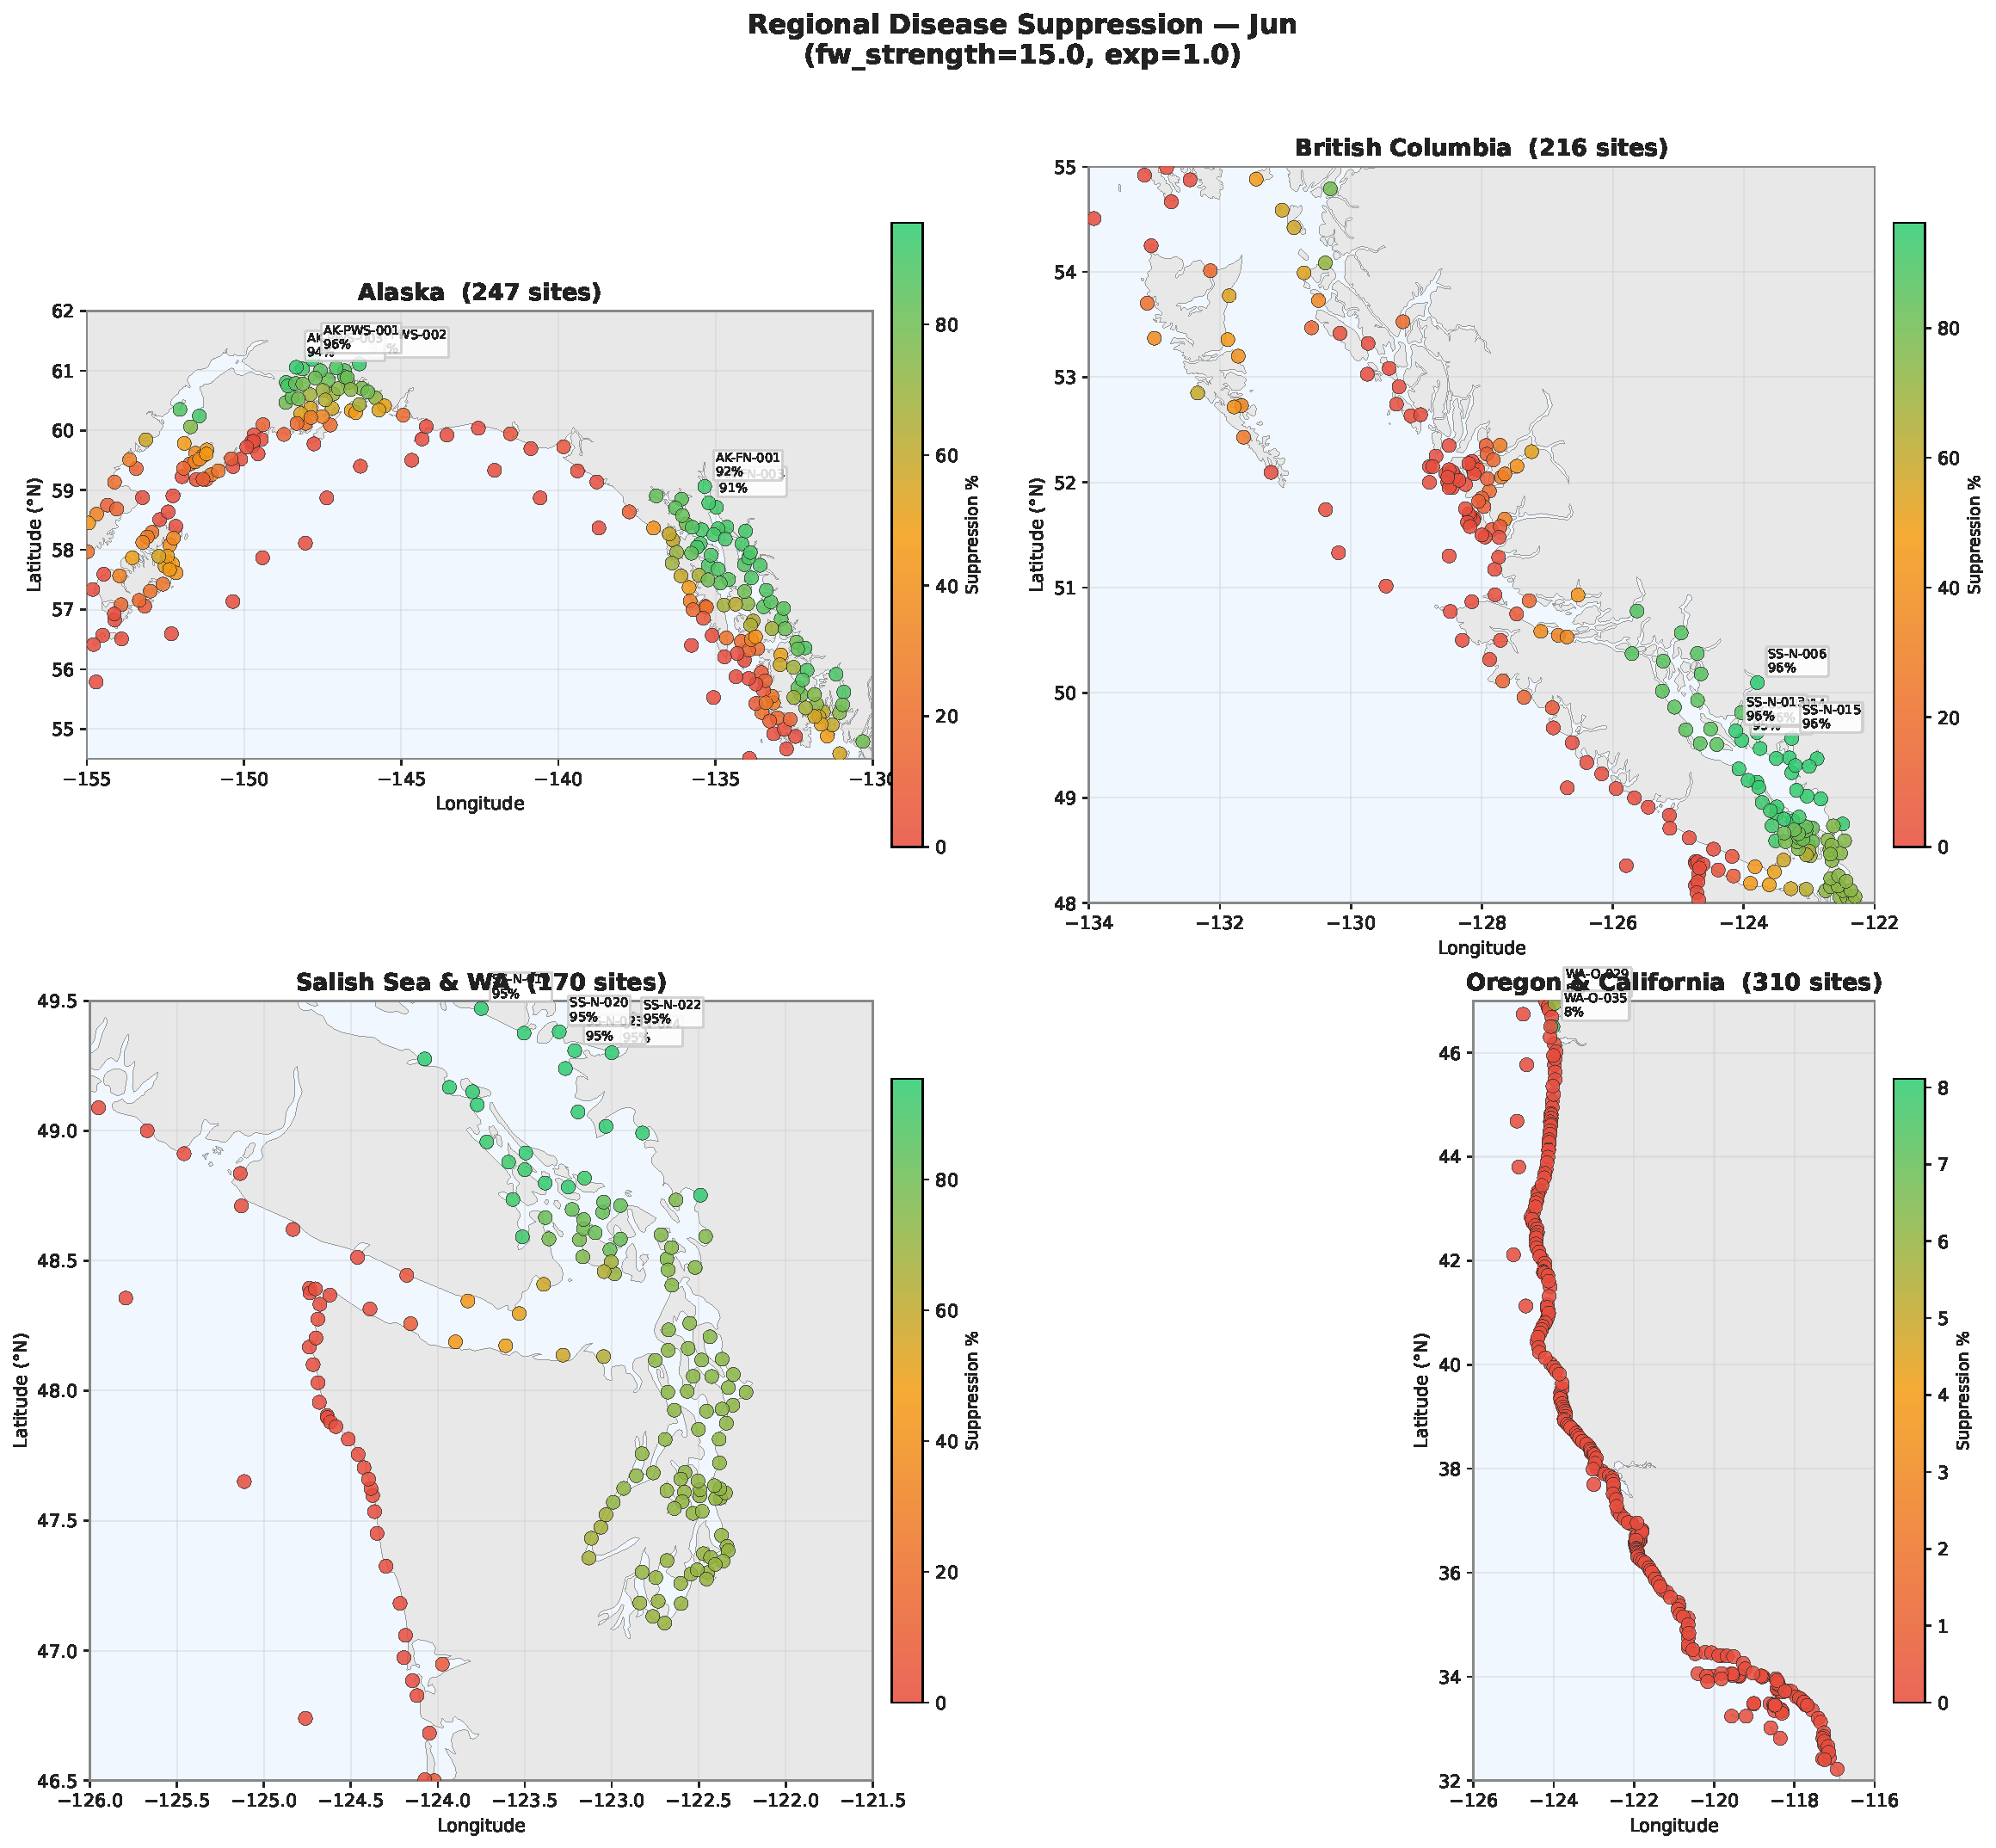
\includegraphics[width=\textwidth]{figures/fig_regional_zoom.pdf}
\caption{Regional disease suppression from salinity in June
(\texttt{fw\_strength=15}). Green = strong suppression (low salinity),
red = no suppression (full-ocean salinity). Coastline polygons from
Natural Earth 10m. Alaska shows concentrated suppression in PWS and
inner fjords; California shows essentially no suppression.}
\label{fig:zoom}
\end{figure}

\subsection{Full Coastline Overview}

Figure~\ref{fig:fullcoast} shows the complete study domain from
Baja California (26.6\textdegree{}N) to the Aleutian Islands
(61.2\textdegree{}N), revealing the strong latitudinal gradient in
disease suppression.

\begin{figure}[H]
\centering
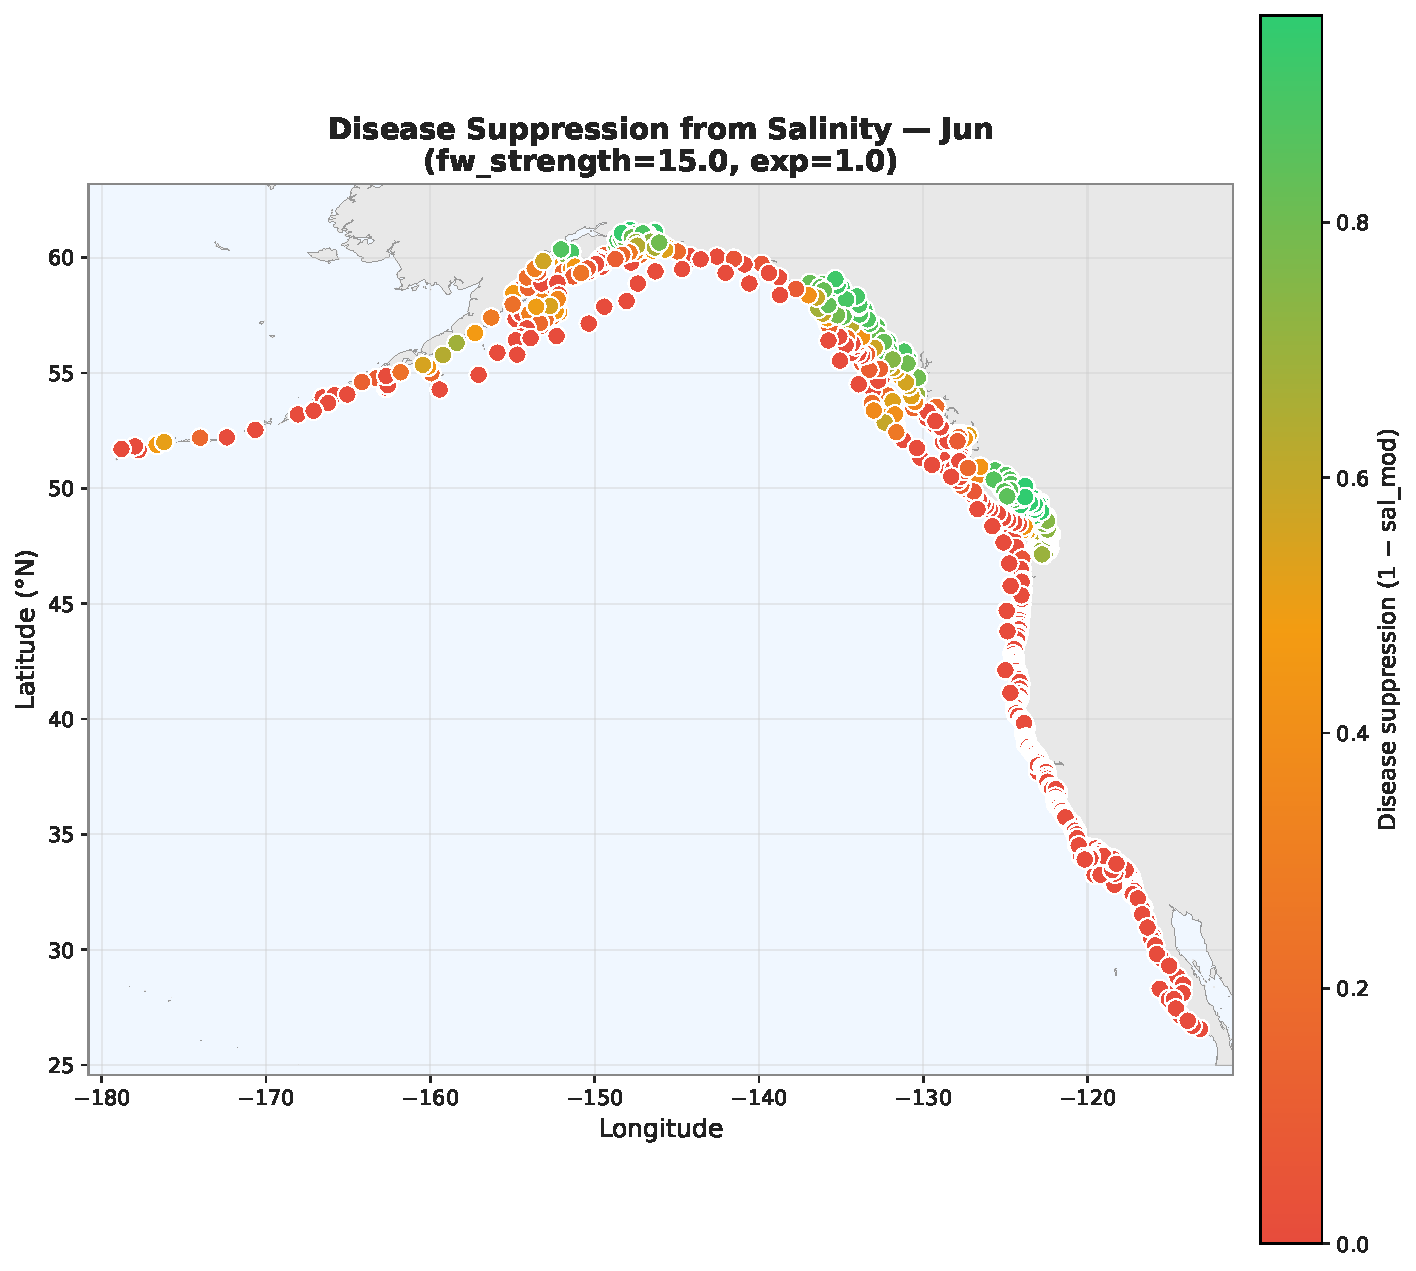
\includegraphics[width=0.65\textwidth]{figures/fig_full_coast.pdf}
\caption{Full-coast disease suppression map, June,
\texttt{fw\_strength=15}. The north-to-south gradient reflects both
$f_\mathrm{melt}(\phi)$ and the concentration of high-enclosedness
sites in Alaska. Sites south of $\sim$40\textdegree{}N show
effectively zero suppression.}
\label{fig:fullcoast}
\end{figure}

\subsection{Regional Salinity Profiles}

Figure~\ref{fig:regional} shows the mean seasonal salinity cycle
for key regions, illustrating how WOA23 differentiates regions that
the parametric model treated identically.

\begin{figure}[H]
\centering
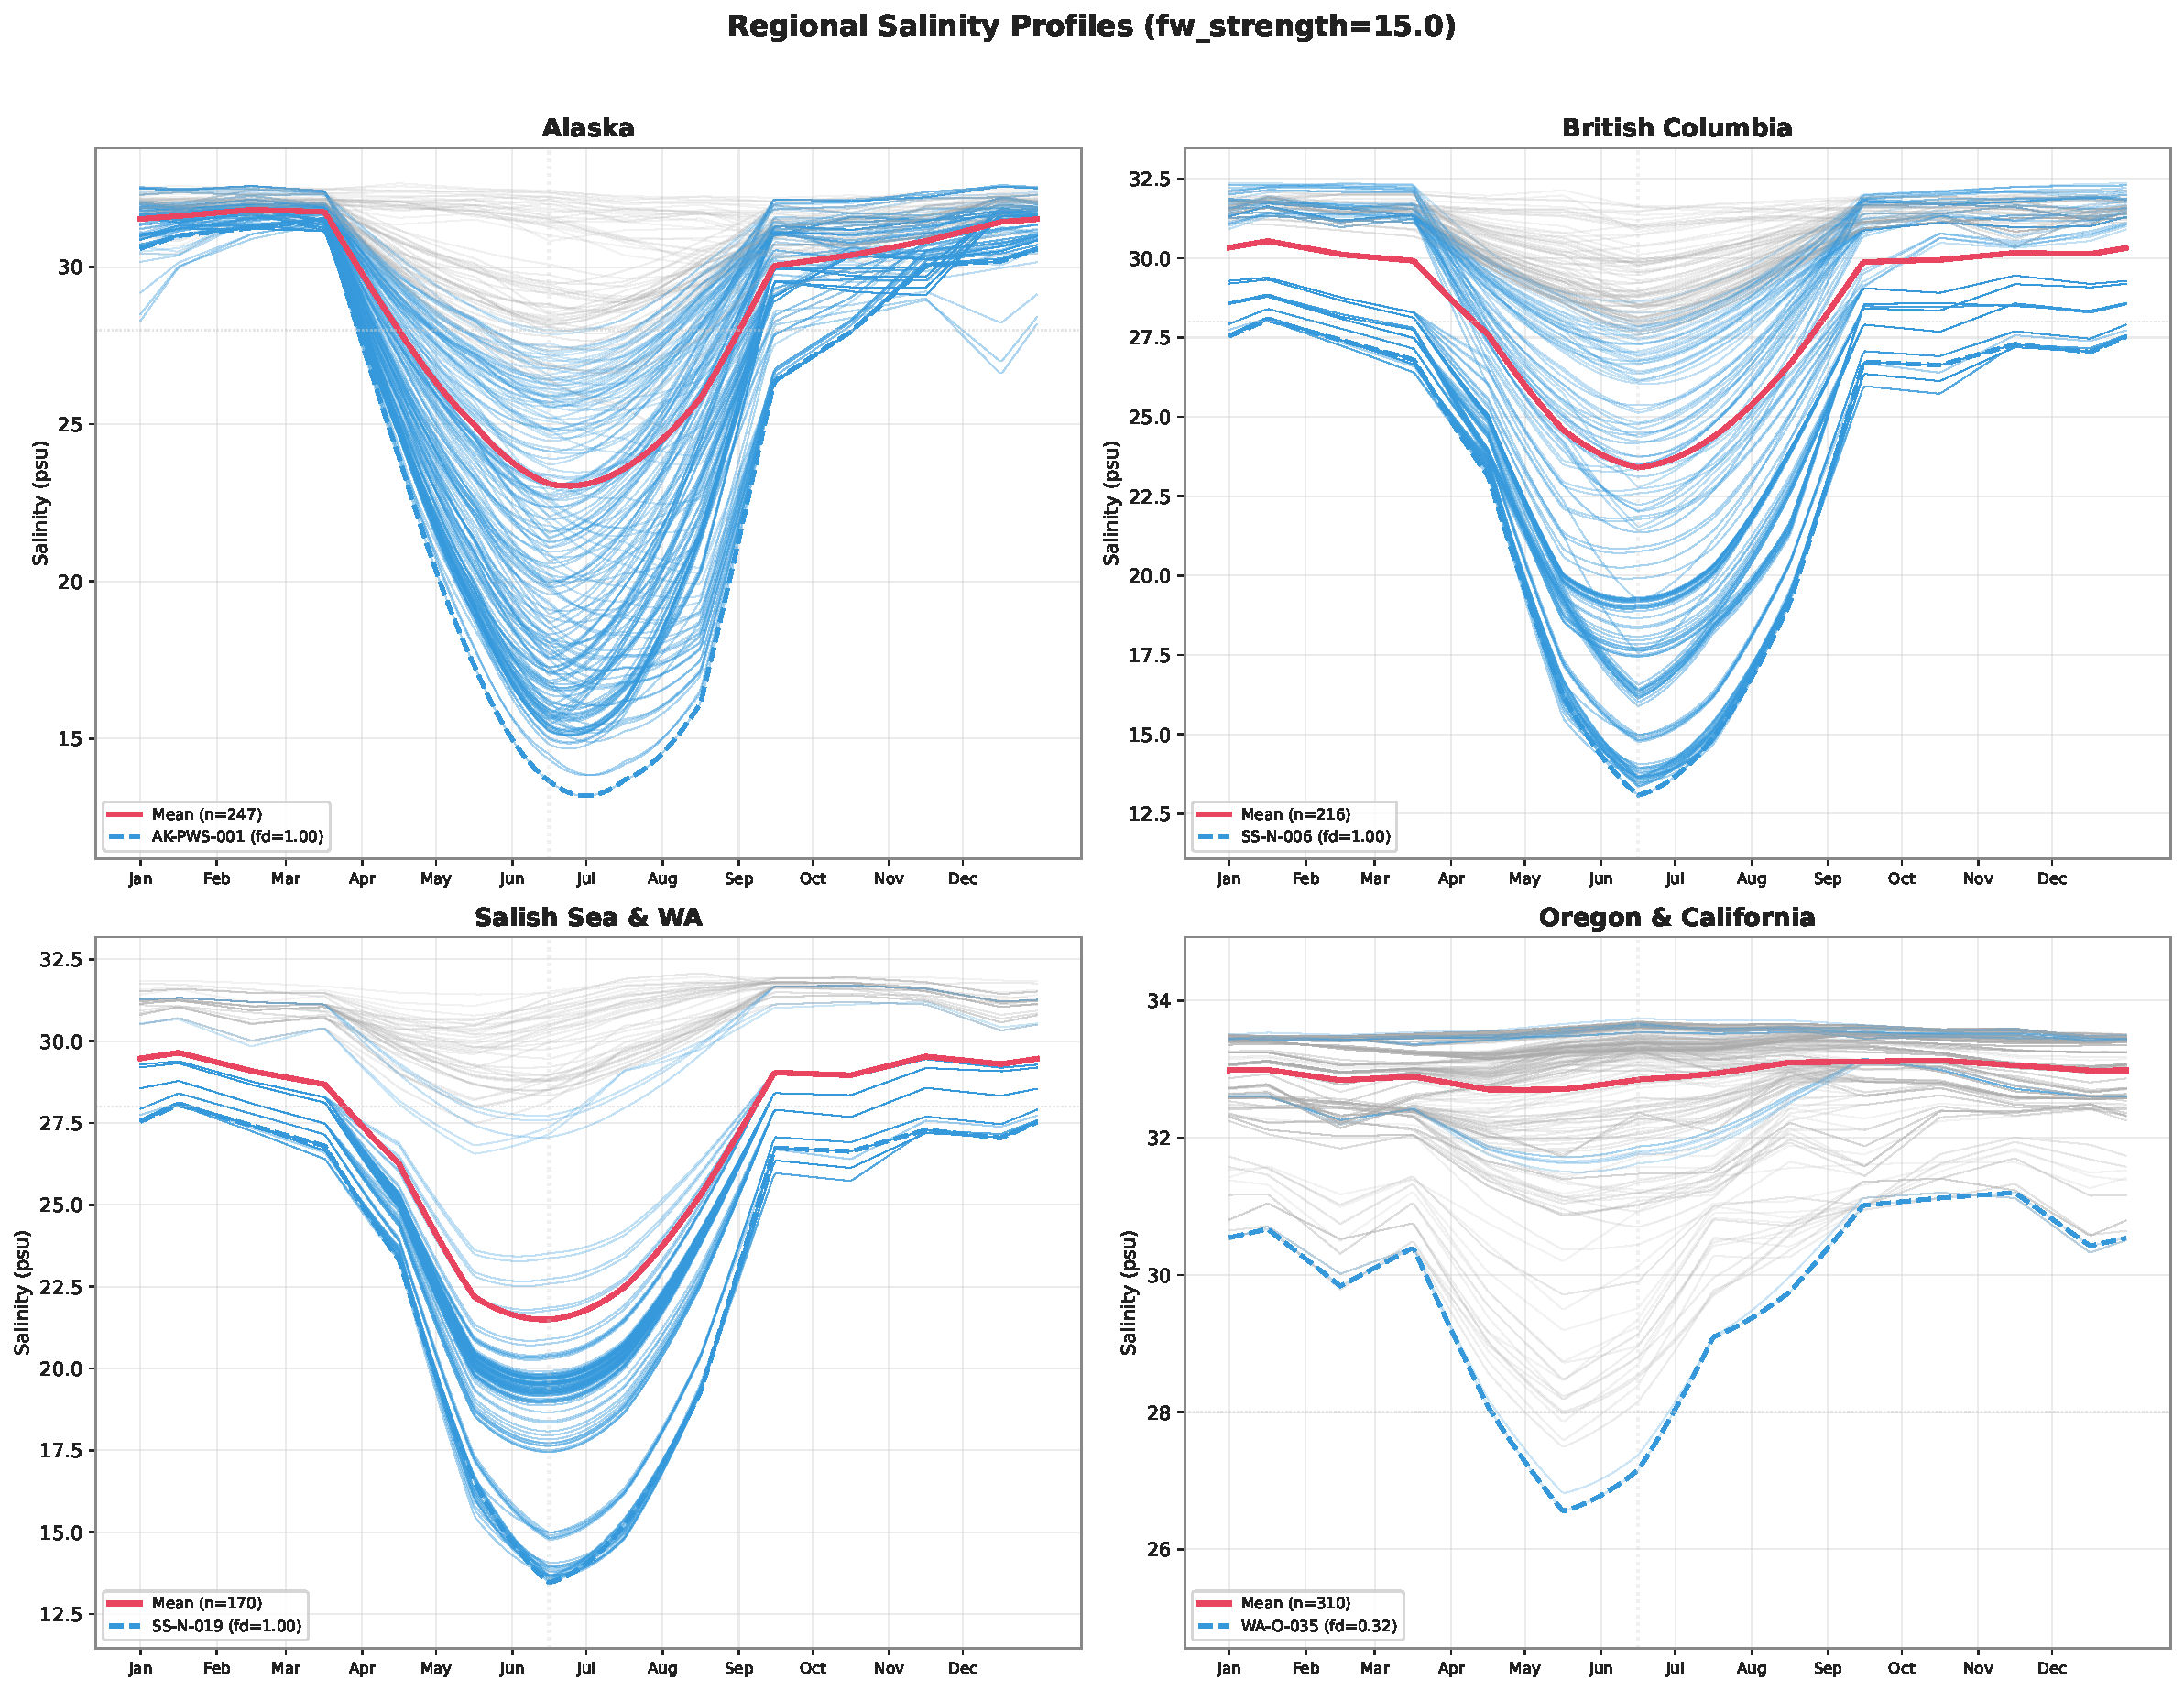
\includegraphics[width=\textwidth]{figures/fig_regional_profiles.pdf}
\caption{Regional seasonal salinity profiles (WOA23 + fjord depression,
\texttt{fw\_strength=15}). Shaded bands show $\pm$1 SD across sites
within each region. Alaska PWS and SE regions show the deepest summer
dips; California and Oregon remain near full-ocean salinity year-round.}
\label{fig:regional}
\end{figure}

\subsection{Freshwater Strength Sensitivity}

Figure~\ref{fig:sensitivity} shows how varying \texttt{fw\_strength}
from 0 to 30~psu affects salinity and disease suppression at
representative sites and across regions.

\begin{figure}[H]
\centering
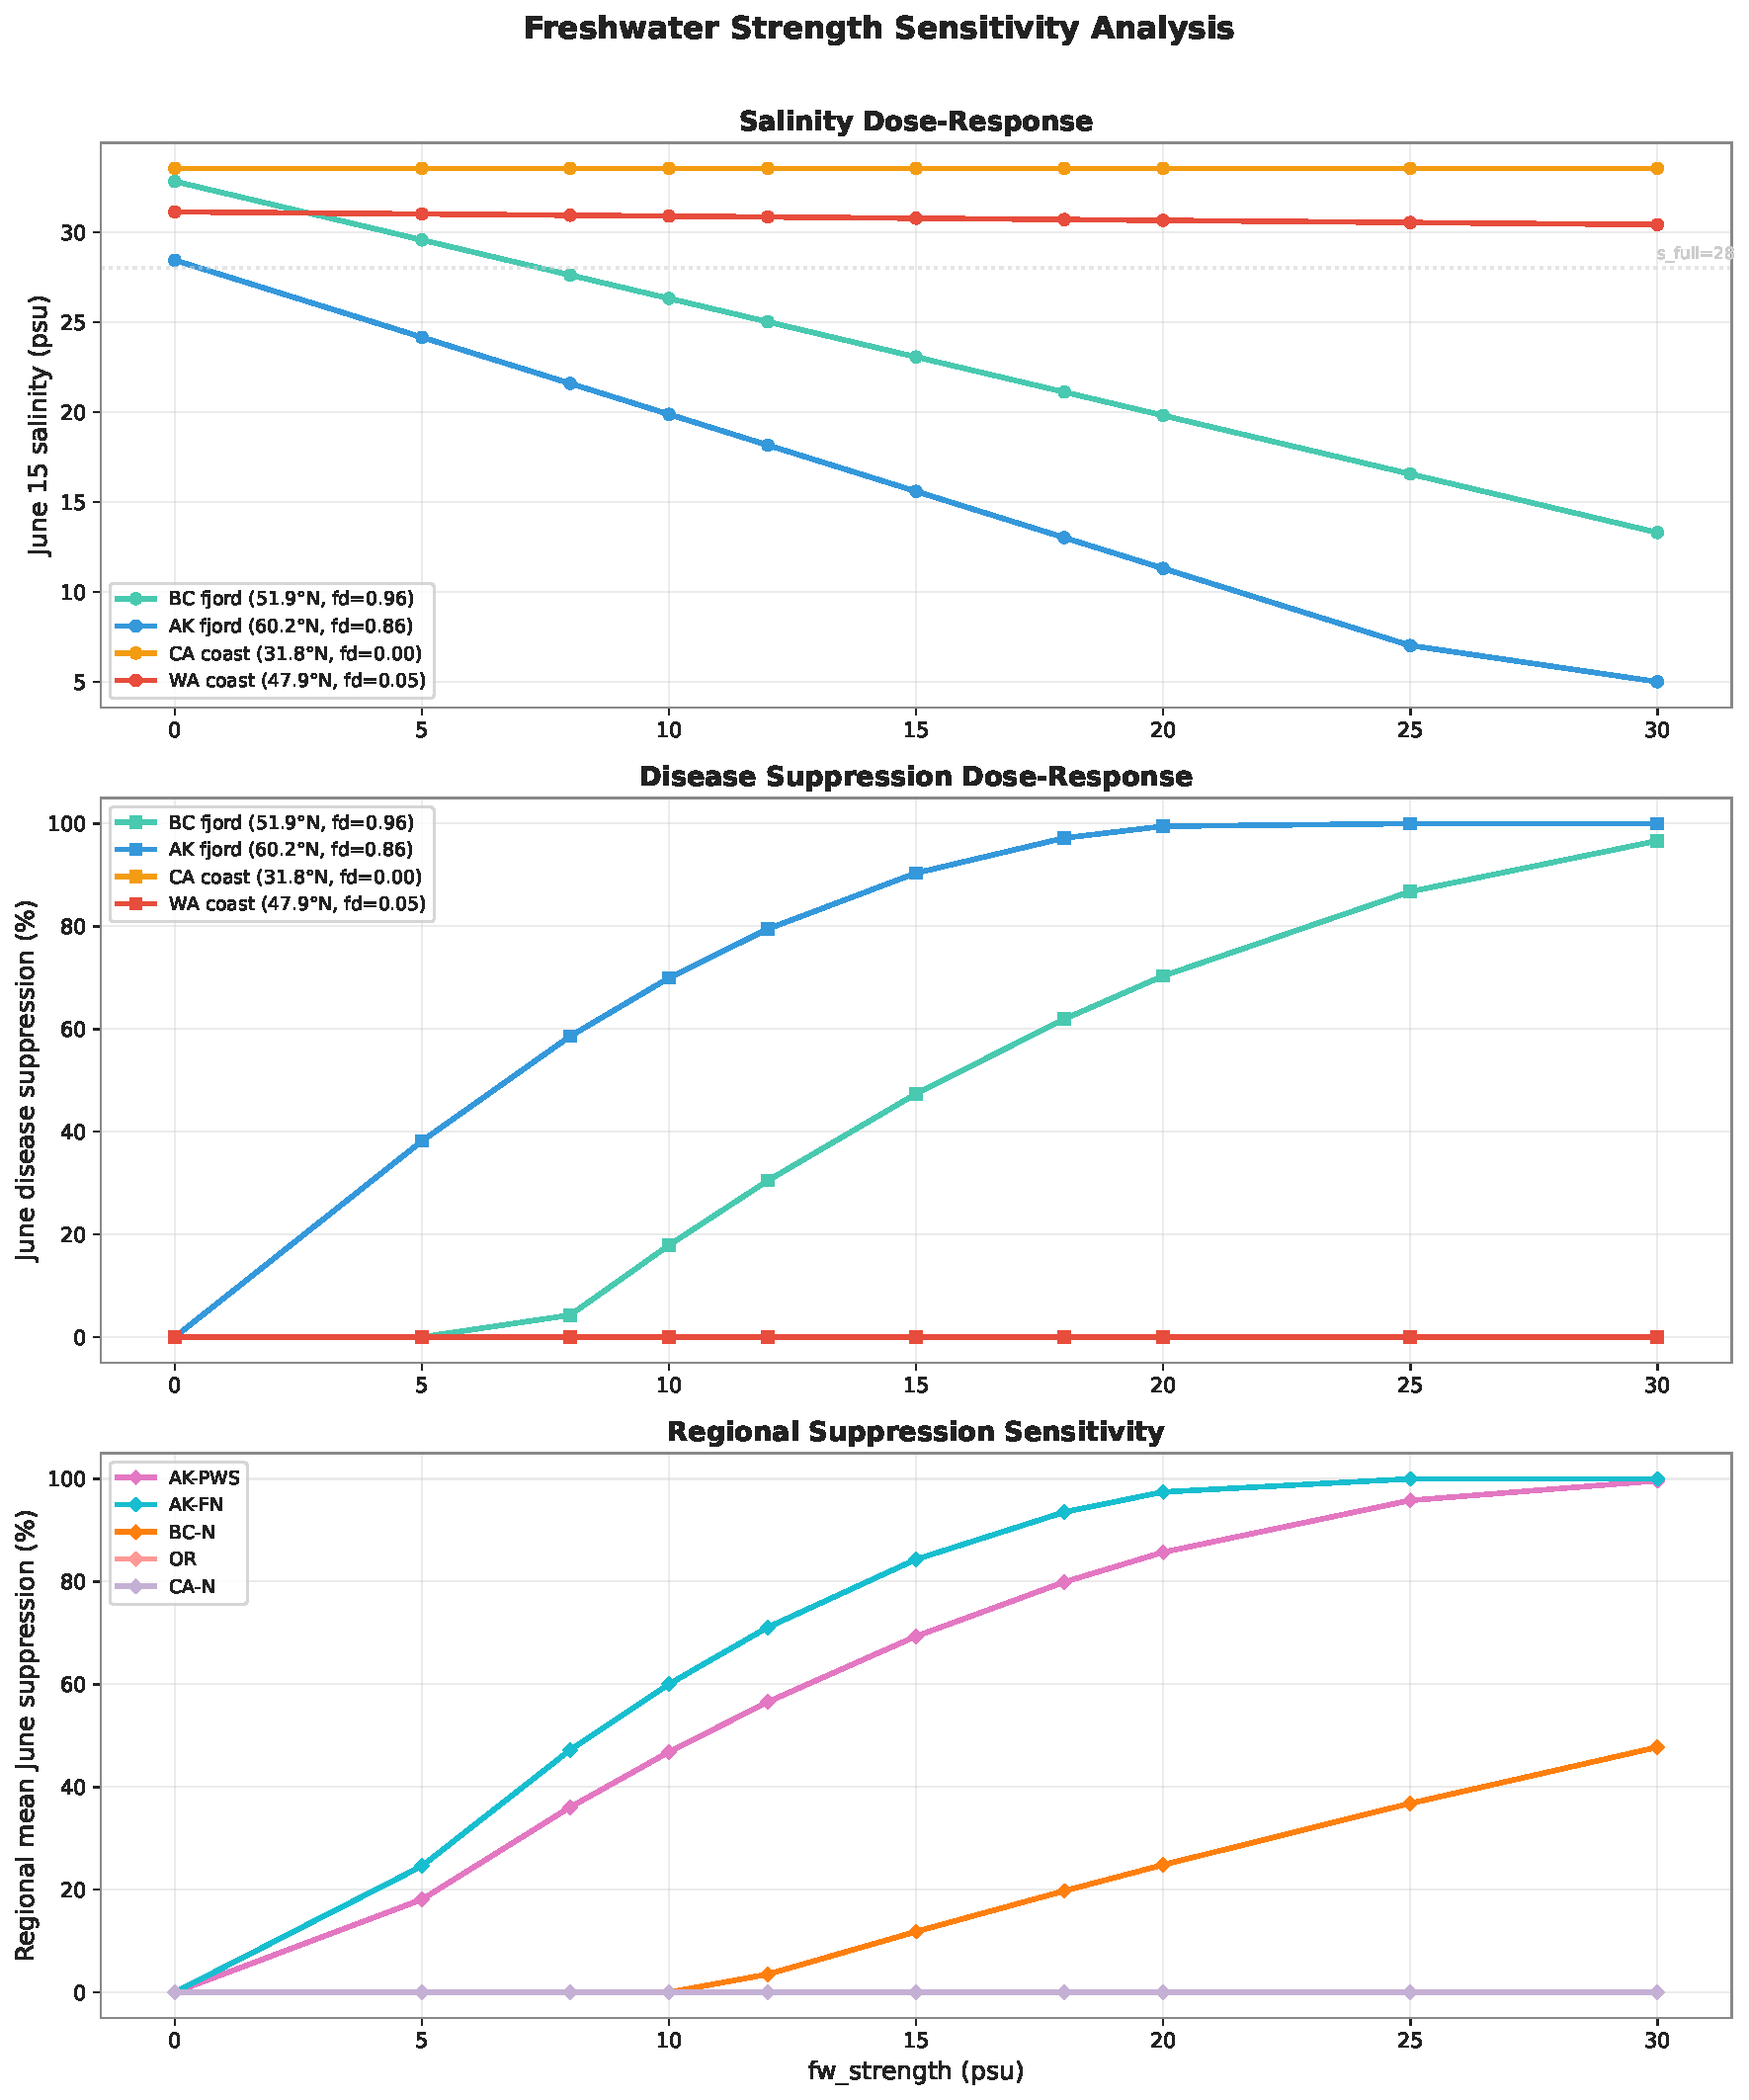
\includegraphics[width=0.9\textwidth]{figures/fig_fw_sensitivity.pdf}
\caption{Sensitivity of June salinity and disease suppression to
\texttt{fw\_strength}. Top: June 15 salinity at four representative
sites. Middle: corresponding disease suppression (\%). Bottom: regional
mean suppression. Alaska fjord sites transition to full suppression
around \texttt{fw=10--15}; California and WA coast sites are unaffected
regardless of \texttt{fw\_strength} (open coast $\times$ low latitude
$= 0$ depression).}
\label{fig:sensitivity}
\end{figure}

% ═══════════════════════════════════════════════════════════════════════
\section{DFO Lighthouse Validation}
% ═══════════════════════════════════════════════════════════════════════

We validated both models against monthly climatological salinity
from 12 Department of Fisheries and Oceans (DFO) lighthouse stations
along the British Columbia coast (48.3--54.3\textdegree{}N),
providing 144 observation-prediction pairs (12 stations $\times$ 12
months).

\begin{figure}[H]
\centering
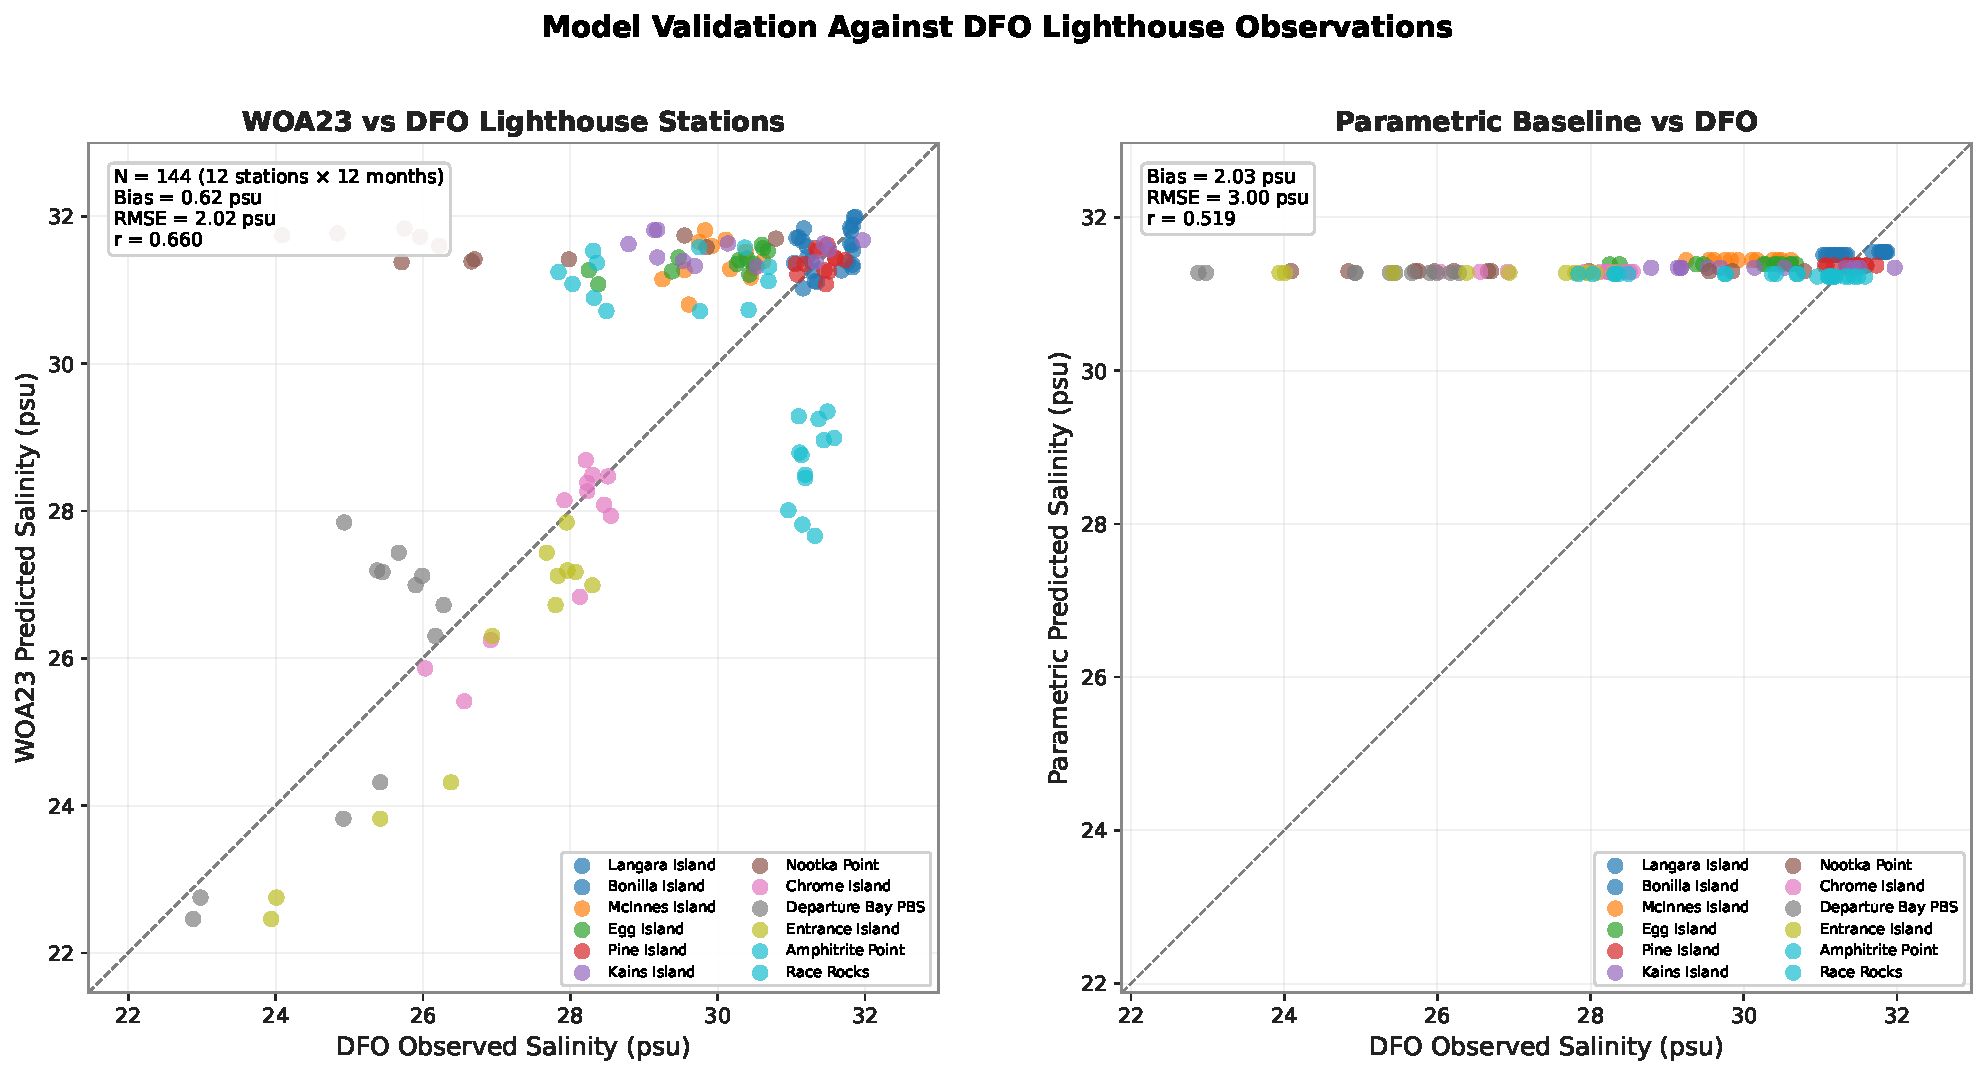
\includegraphics[width=\textwidth]{figures/fig_dfo_validation.pdf}
\caption{Model validation against DFO lighthouse stations. Left: WOA23
predictions vs.\ observations. Right: parametric predictions vs.\
observations. WOA23 shows improved correlation ($r=0.660$ vs.\ 0.519)
and reduced RMSE (2.02 vs.\ 3.00~psu). Note that DFO stations are on
headlands (\texttt{fjord\_depth\_norm}$\approx$0), so only the WOA23
baseline layer is evaluated here.}
\label{fig:dfo}
\end{figure}

\begin{table}[H]
\centering
\caption{DFO lighthouse validation summary (12 stations, 144 points).}
\label{tab:dfo}
\begin{tabular}{lccc}
\toprule
\textbf{Metric} & \textbf{WOA23} & \textbf{Parametric} & \textbf{Improvement} \\
\midrule
Mean bias (psu)   & 0.62  & 2.03  & 69\% lower \\
RMSE (psu)        & 2.02  & 3.00  & 33\% lower \\
Correlation ($r$) & 0.660 & 0.519 & +0.141 \\
Max error (psu)   & 7.65  & ---   & --- \\
\bottomrule
\end{tabular}
\end{table}

The WOA23 model outperforms the parametric baseline on all three
metrics. The remaining RMSE of 2.02~psu is dominated by a few
stations with strong local freshwater influence (e.g., Nootka Point,
Departure Bay) where even WOA23's 0.25\textdegree{} resolution
cannot fully resolve the coastal gradient. These are precisely the
sites where Layer~2 (fjord depression) would apply in the full model.

% ═══════════════════════════════════════════════════════════════════════
\section{Implications for Calibration}
% ═══════════════════════════════════════════════════════════════════════

The transition from parametric to WOA23 baseline has several important
implications for model calibration:

\begin{enumerate}
    \item \textbf{Reduced \texttt{fw\_strength} requirement}: Because
    WOA23 already captures much of the coastal freshwater signal (seasonal
    range 1.68~psu), the Layer~2 depression need only represent the
    \emph{residual} sub-grid freshwater---likely requiring a lower
    \texttt{fw\_strength} than the parametric-only model.

    \item \textbf{Regional timing realism}: The parametric model applied
    the same June-peaked cosine pulse everywhere. WOA23 provides
    region-specific seasonal timing automatically. The remaining Layer~2
    pulse still peaks uniformly at June~15, but its contribution is
    smaller, reducing the impact of this assumption.

    \item \textbf{Salish Sea correction}: The parametric model assigned
    $\sim$31~psu to Puget Sound sites (based on latitude alone). WOA23
    correctly identifies salinities of 25--28~psu, fundamentally changing
    the disease dynamics in this critical region.

    \item \textbf{California salinity increase}: WOA23 places California
    sites at 33--34~psu (vs.\ $\sim$30~psu parametric), reducing
    any spurious freshwater suppression in the south.

    \item \textbf{Calibration target}: The \texttt{fw\_strength} sweep
    should now explore a range of 0--20~psu (vs.\ 0--30~psu previously),
    with the expectation that optimal values will be lower since the
    baseline already contains seasonal variation.
\end{enumerate}

% ═══════════════════════════════════════════════════════════════════════
\section{Limitations}
% ═══════════════════════════════════════════════════════════════════════

\begin{enumerate}
    \item \textbf{Nearest-neighbor fill}: 661 of 896 sites (73.8\%)
    use nearest-neighbor fill from WOA23 ocean cells rather than
    direct grid-cell extraction. While the maximum NN distance is only
    0.177\textdegree{} ($\approx$19.6~km), this means inland and
    deep-fjord sites receive salinities from the nearest open-ocean
    cell, potentially overestimating their baseline.

    \item \textbf{Uniform pulse timing}: The Layer~2 cosine depression
    pulse peaks at day 166 (June~15) for all sites, regardless of local
    hydrology. In reality, peak freshwater discharge varies by weeks
    across the study domain. This is partially mitigated by WOA23
    already capturing the site-specific timing in Layer~1.

    \item \textbf{Resolution limits}: WOA23 at 0.25\textdegree{}
    ($\approx$28~km) cannot resolve narrow channels, small inlets,
    or micro-fjords. Sites deep within complex coastlines may have
    WOA23 values biased toward open-ocean conditions.

    \item \textbf{Climatological vs.\ interannual}: WOA23 provides a
    long-term climatological mean, not year-specific conditions.
    Anomalous years (e.g., marine heatwaves, strong El Ni\~{n}o)
    are not represented.

    \item \textbf{DFO validation geography}: All 12 DFO lighthouse
    stations are in British Columbia (48--54\textdegree{}N). We lack
    independent validation data for Alaska and California, the regions
    where WOA23 diverges most from the parametric model.
\end{enumerate}

% ═══════════════════════════════════════════════════════════════════════
\section*{Appendix: Model Parameters}
% ═══════════════════════════════════════════════════════════════════════

\begin{table}[H]
\centering
\caption{Model parameters and defaults.}
\begin{tabular}{llll}
\toprule
\textbf{Parameter} & \textbf{Symbol} & \textbf{Default} & \textbf{Description} \\
\midrule
\texttt{fw\_strength}   & $f_\mathrm{fw}$ & 0.0    & Freshwater depression strength (psu) \\
\texttt{fw\_depth\_exp} & exp              & 1.0    & Exponent on fjord depth norm \\
\texttt{s\_floor}       & $S_\mathrm{floor}$ & 5.0  & Physical minimum salinity (psu) \\
\texttt{s\_min}         & ---              & 10.0   & Vibrio zero-activity threshold (psu) \\
\texttt{s\_full}        & ---              & 28.0   & Vibrio full-activity threshold (psu) \\
Peak day                & ---              & 166    & Day of year for melt pulse peak \\
\bottomrule
\end{tabular}
\end{table}

\end{document}
